\documentclass[tikz,border=2pt]{standalone}
\usepackage{pgfplots}
\usepgfplotslibrary{fillbetween,groupplots}
\pgfplotsset{compat=1.18}
\begin{document}
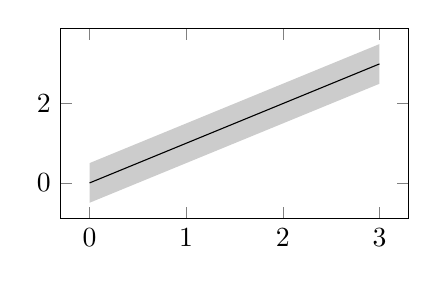
\begin{tikzpicture}
\begin{axis}[width=6cm,height=4cm]
\addplot[name path=upper,draw=none,domain=0:3] {x+0.5};
\addplot[name path=lower,draw=none,domain=0:3] {x-0.5};
\addplot[opacity=0.2] fill between[of=upper and lower];
\addplot[domain=0:3] {x};
\end{axis}
\end{tikzpicture}

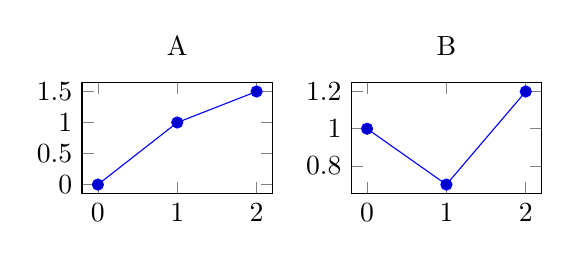
\begin{tikzpicture}
\begin{groupplot}[group style={group size=2 by 1},width=4cm,height=3cm]
\nextgroupplot[title={A}]
\addplot coordinates {(0,0) (1,1) (2,1.5)};
\nextgroupplot[title={B}]
\addplot coordinates {(0,1) (1,0.7) (2,1.2)};
\end{groupplot}
\end{tikzpicture}
\end{document}
